\section{Profiling and Optimization}
In this section, I performed profiling and optimization on the IBP linear-Gaussian model. The optimization strategies include removing redundant calculations, better use of matrix multiplication, cythonizing Python code, and using the jit (just-in-time) compiler. Since the MCMC chain posesses the Markov property; that is, the $n$th sample only depends on the $(n-1)$th sample, it is unreasonable to parallelize the IBP code.

\subsection{Profiling}
The code structure can be visualized as a tree in Figure~\ref{fig:profiling}, and profiling is done to identify the bottlenecks. In one Gibbs sampling iteration, generating $Z|\alpha$ and sampling $\sigma_X,\sigma_A$ are performed once each. In generating $Z|\alpha$, sampling dishes from $K_+$ and sampling new dishes are done for each customer (image or object), so they are each performed $N=100$ times. In sampling dishes from $K_+$, calculation refers to the process of sampling the posterior distribution of $Z|K_+$, and initialization is the part of removing features which are all zero. Both calculation and initialization are performed $N\times K_+ \approx 500$ times for each iteration.\\

Table~\ref{tab:naive} shows the profiling results for my initial code. The calculation in sampling from $K_+$ for generating $Z|\alpha$ accounts for about 70\% of the time, approximately 1.4 seconds per iteration because it involves matrix inversion and likelihood calculation. Matrix inversion and determinant calculation are notoriously slow; they run between $O(n^2)$ and $O(n^3)$.

\begin{figure}[!ht]
\centering
    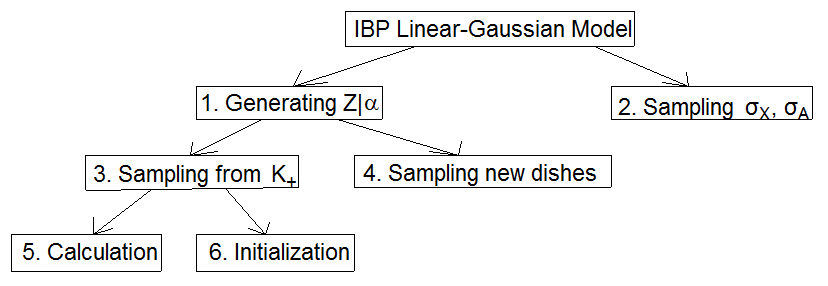
\includegraphics[width=\linewidth]{More_Images/IBP_profiling.png}
    %\vspace{-20pt}
    \caption{IBP code structure for profiling}
    \label{fig:profiling}
\end{figure}

\subsection{Remove Redundant Calculations}
\label{sub:usable}
To optimize the code, redundant calculations are removed first, and this version is named as "usable". When generating $Z|\alpha$, the inverted matrix $\mathbf{M} = (\mathbf{Z}^T\mathbf{Z}+\dfrac{\sigma_X^2}{\sigma_A^2}\mathbf{I})^{-1}$ is only calculated directly before the likelihood computation, so more than $N = 100$ matrix inversions can be removed. The speed of generating $Z|\alpha$ is improved by 1.5\%, equivalent to 0.023 seconds per iteration, so this "usable" code is at least 23 seconds faster than the initial version. The profiling results are shown in Table~\ref{tab:usable}. 

\subsection{Matrix Multiplication}
% Dynamic programming -- the order of matrix multiplication matters
Matrix multiplication is associative, say $(\mathbf{A}\mathbf{B})\mathbf{C} = \mathbf{A}(\mathbf{B}\mathbf{C})$, but the order of multiplication can affect the computation speed. According to dynamic programming~\cite{matrixmult}, here is an example of how this works: The dimensions of matrices $\mathbf{A},\mathbf{B},\mathbf{C}$ are $4 \times 2,2 \times 5, 5 \times 1$, respectively.
\begin{itemize}
\item $(\mathbf{A}\mathbf{B})\mathbf{C}$: total multiplications = $4 \times 2 \times 5 + 4 \times 5 \times 1 = 60$
\item $\mathbf{A}(\mathbf{B}\mathbf{C})$: total multiplications = $2 \times 5 \times 1 + 4 \times 2 \times 1 = 18$
\end{itemize}
As a result, the order of multiplications can make a huge difference in computation.\\

In my IBP code, some matrix multiplications have the potential to be computed faster, but it turned out that either I have already selected the faster way, or the number of total multiplications are the same for both methods. First, to calculate the resulting features matrix $\mathbf{A}_{\text{inf}} = (\mathbf{Z}^T\mathbf{Z}+\dfrac{\sigma_X^2}{\sigma_A^2}\mathbf{I})^{-1}\mathbf{Z}^T \mathbf{X}$, I can start from either the first two or the last two matrices. $\mathbf{Z}$ has size $N \times K_+ = 100 \times 4$; hence the first term $\mathbf{M} = (\mathbf{Z}^T\mathbf{Z}+\dfrac{\sigma_X^2}{\sigma_A^2}\mathbf{I})^{-1}$ has size $K_+ \times K_+ = 4 \times 4$; the second term $\mathbf{Z}^T$ has size $K_+ \times N = 4 \times 100$, and the third term $\mathbf{X}$ has size $N \times D = 100 \times 36$.

% Make use of different colors to show this with \usepackage{color}: {\color{declared-color} some text}
\begin{itemize} 
\item $(\mathbf{M}\mathbf{Z}^T) \mathbf{X}$: total multiplications = ${\bf{4 \times 4 \times 100}} + 4 \times 100 \times 36$
\item $\mathbf{M} (\mathbf{Z}^T\mathbf{X})$: total multiplications = ${\bf{4 \times 4 \times 36}} + 4 \times 100 \times 36$
\end{itemize}
Multiplying $\mathbf{Z}^T$ and $\mathbf{X}$ first is faster than doing the other way.\\

In addition to $\mathbf{A}_{\text{inf}}$, the kernel of the log-likelihood function involves calculating $\mathbf{X}^T (\mathbf{I} - \mathbf{Z}\mathbf{M}\mathbf{Z}^T)\mathbf{X}$. However, the middle term $(\mathbf{I} - \mathbf{Z}\mathbf{M}\mathbf{Z}^T)$ is a $100 \times 100$ square matrix, so multiplying the three matrices in either order requires $36 \times 100 \times 100 \times 2$ multiplications.

\subsection{Cythonized Code}
% Vectorization, calInverse
The "usable" version code can also be cythonized (converted from Python to C), and Table~\ref{tab:cythonized} is a summary of profiling results, but the Cythonized version only improved the speed about 1.5\%.

\subsection{Using jit (just-in-time compiler)}

The jit (just-in-time compiler) is from the Python package \texttt{numba}, which generates optimized machine code from the LLVM compiler infrastructure. The jit in Python is claimed to have similar performance to C/C++ without switching languages~\cite{numba}. The speed comparison table is shown in Table~\ref{tab:jit}, but this version performs almost the same as the Python "usable" version.

% Z|alpha: 7.5% improvement from the initial code, 5.2% improvement from the usable code.
% In fact, using jit (just-in-time compiler) to compile the $\mathbf{M}$ and log-likelihood calculation functions gives the best results of all four versions in speed. The execution time of generating $Z|\alpha$ is 7.5\% less than the initial code, and 5.2\% less than the "usable" version in Section~\label{sub:usable}.

\subsection{Comparison Tables}
All four tables summarizing which actions take how much time are here for ease of comparison.

% A table to summarize which actions take how much time.
% Don't add minipage in front of tables!
\begin{table}[!ht]
  \centering
  \begin{tabular}{lrrr}
\toprule
{} &  Time (seconds)/action &  Times performed &  Total time (seconds) \\
\midrule
Generating Z given alpha &               1.598608 &                1 &              1.598608 \\
Sampling sigmaX, sigmaA  &               0.003846 &                1 &              0.003846 \\
Sampling from K+         &               0.011336 &              100 &              1.133637 \\
Sampling new dishes      &               0.004551 &              100 &              0.455109 \\
Calculation              &               0.002416 &              500 &              1.208202 \\
Initialization           &               0.000007 &              500 &              0.003707 \\
\bottomrule
\end{tabular}

  \caption{Initial code: Profiling results per iteration}
  \label{tab:naive}
\end{table}

\begin{table}[!ht]
  \centering
  \begin{tabular}{lrrr}
\toprule
{} &  Time (seconds)/action &  Times performed &  Total time (seconds) \\
\midrule
Generating Z given alpha &               1.572500 &                1 &              1.572500 \\
Sampling sigmaX, sigmaA  &               0.003756 &                1 &              0.003756 \\
Sampling from K+         &               0.011194 &              100 &              1.119370 \\
Sampling new dishes      &               0.004529 &              100 &              0.452930 \\
Calculation              &               0.002219 &              500 &              1.109398 \\
Initialization           &               0.000007 &              500 &              0.003420 \\
\bottomrule
\end{tabular}

  \caption{Usable code: Profiling results per iteration}
  \label{tab:usable}
\end{table}

\begin{table}[!ht]
  \centering
  \begin{tabular}{lrrr}
\toprule
{} &  Time (seconds)/action &  Times performed &  Total time (seconds) \\
\midrule
Generating Z given alpha &               1.575697 &                1 &              1.575697 \\
Sampling sigmaX, sigmaA  &               0.003630 &                1 &              0.003630 \\
Sampling from K+         &               0.011202 &              100 &              1.120241 \\
Sampling new dishes      &               0.004552 &              100 &              0.455236 \\
Calculation              &               0.002233 &              500 &              1.116524 \\
Initialization           &               0.000007 &              500 &              0.003602 \\
\bottomrule
\end{tabular}

  \caption{Cythonized code: Profiling results per iteration}
  \label{tab:cythonized}
\end{table}

\begin{table}[!ht]
  \centering
  \begin{tabular}{lrrr}
\toprule
{} &  Time (seconds)/action &  Times performed &  Total time (seconds) \\
\midrule
Generating Z given alpha &               1.575537 &                1 &              1.575537 \\
Sampling sigmaX, sigmaA  &               0.005048 &                1 &              0.005048 \\
Sampling from K+         &               0.011275 &              100 &              1.127496 \\
Sampling new dishes      &               0.004478 &              100 &              0.447848 \\
Calculation              &               0.002384 &              500 &              1.192065 \\
Initialization           &               0.000007 &              500 &              0.003296 \\
\bottomrule
\end{tabular}

  \caption{Using jit (just-in-time compiler): Profiling results per iteration}
  \label{tab:jit}
\end{table}